\documentclass[a4paper,12pt]{article}

% --- Encoding and Fonts ---
\usepackage[utf8]{inputenc}
\usepackage{mathptmx} % Times New Roman font

% --- Page Layout ---
\usepackage{geometry}
\geometry{
    a4paper,
    left=1.5in,
    right=1.25in,
    top=1in,
    bottom=1in,
    headheight=0.5in,
    headsep=0.5in,
    footskip=0.5in
}

% --- Graphics and Tables ---
\usepackage{graphicx}
\usepackage{array}
\usepackage{caption}
\usepackage{tikz}
\usepackage{enumitem}  % unordered list
\usetikzlibrary{arrows.meta, positioning, calc}

% --- Formatting and Spacing ---
\usepackage{setspace}
\setstretch{1.5}


% --- Footer Only (Page Number) ---
\usepackage{fancyhdr}
\pagestyle{fancy}
\fancyhf{}
\renewcommand{\headrulewidth}{0pt}
\fancyfoot[C]{\thepage}

\usepackage{titlesec}
\titleformat{\section}
  {\normalfont\bfseries\fontsize{18}{22}\selectfont}{\thesection}{1em}{}
\titleformat{\subsection}
  {\normalfont\bfseries\fontsize{16}{19}\selectfont}{\thesubsection}{1em}{}
\titleformat{\subsubsection}
  {\normalfont\bfseries\fontsize{14}{17}\selectfont}{\theparagraph}{1em}{}
\titleformat{\paragraph}[runin]
  {\normalfont\bfseries\fontsize{13}{15}\selectfont}{\theparagraph}{1em}{}

% --- Hyperlinks ---
\usepackage{hyperref}
\hypersetup{
    colorlinks=true,
    linkcolor=blue,
    urlcolor=blue,
    pdftitle={Digital Logic Suite Proposal},
    pdfauthor={},
    pdfsubject={Project Proposal}
}

% --- Document ---
\begin{document}

\begin{titlepage}
    \begin{center}
        % University Logo
        
\includegraphics[width=3.5cm]{images/tuLogo.png}
        \vspace{0.8cm}

        % University Name
        {\large TRIBHUVAN UNIVERSITY} \\
        {\normalsize INSTITUTE OF ENGINEERING} \\
        {\normalsize PULCHOWK CAMPUS}
        \vspace{1cm}

        % Title
        {\large A PROJECT REPORT ON} \\
        \vspace{0.4cm}
        {\LARGE \textbf{DIGITAL LOGIC SIMULATOR}} \\
        \vspace{0.2cm}
        {\normalsize \textit{\textbf{GUI BASED TOOL}}}
        \vspace{1cm}

        % Submitted By
        {\normalsize \textbf{SUBMITTED BY:}} \\
        \vspace{0.2cm}
        {\normalsize NABARAJ BHANDARI (081BCT041)} \\
        {\normalsize NIKUNJ BHUSAL (081BCT043)} \\
        {\normalsize NIRDESH JOSHI (081BCT044)}
        \vspace{0.8cm}

        % Supervised By
        {\normalsize \textbf{SUPERVISED BY:}} \\
        \vspace{0.2cm}
        {\normalsize SENIOR FACULTY MEMBER, DAYA SAGAR BARAL}
        \vspace{0.8cm}

        % Submitted To
        {\normalsize \textbf{SUBMITTED TO:}} \\
        \vspace{0.2cm}
        {\normalsize DEPARTMENT OF ELECTRONICS AND COMPUTER ENGINEERING} \\
        {\normalsize INSTITUTE OF ENGINEERING, PULCHOWK CAMPUS}
        \vspace{1cm}

        % Submission Date
        {\normalsize \textbf{SUBMISSION DATE:}} \\
        \vspace{0.2cm}
        {\normalsize 2082 Bhadra 02, Monday}
    \end{center}
\end{titlepage}
\clearpage

\pagenumbering{roman}
\phantomsection
\addcontentsline{toc}{section}{Acknowledgement.tex}
\section*{Acknowledgment}

We would like to express our sincere gratitude to our supervisor, \textbf{Mr. Daya Sagar Baral}, Senior Faculty Member, Department of Electronics and Computer Engineering, IOE Pulchowk Campus, for his amazing guidance, helpful feedback, and constant support. His knowledge of programming and digital logic helped us understand and build this project better.

\vspace{0.5cm}
This project, \textbf{Digital Logic Simulator}, has been carried out as part of the subject \textbf{Object-Oriented Programming with C++}, and it would not have been possible without the support provided by our supervisor. His expertise and insights have greatly contributed to the successful design and implementation of this project.

\vspace{0.5cm}
We extend our sincere thanks to the faculty members of the Department of Electronics and Computer Engineering at Pulchowk Campus for providing us with the necessary resources and an excellent learning environment. Their lectures on C++ programming were really helpful for this project. Our heartfelt appreciation goes to our classmates and friends who offered constructive suggestions during its development phases.

\vspace{0.5cm}
Finally, we thank Tribhuvan University for including projects in our studies, letting us use what we learned in a real project. This work has greatly improved our skills in C++ programming, software design, and working as a team.
\clearpage
\section*{Abstract}
The Digital Logic Suite is a user-friendly app built with C++ and SFML (Simple Fast Multimedia Library) to provide features like designing, testing, and studying digital logic circuits. It uses object-oriented programming ideas to make a helpful tool for students.

\vspace{0.5cm}
Users can place logic gates like AND, OR, NOT, INPUT, and OUTPUT, then connect them with wires to build circuits. This application can be used to see how circuits work in real time and makes truth tables for the designs. Users can also enter Boolean expressions and see their simplified form on the screen.

\vspace{0.5cm}
This tool is a lighter option compared to expensive software, works well on different systems, and includes key features for learning digital logic. The project shows how to use C++ programming effectively and sets the stage for future improvements in circuit simulation.
\clearpage
\clearpage

\phantomsection
\addcontentsline{toc}{section}{Table of Contents}
\renewcommand{\contentsname}{Table of Contents}
\tableofcontents
\clearpage

\pagenumbering{arabic}
\section{Objectives}

The primary objective of the \textbf{Digital Logic Suite} project is to develop a practical GUI-based tool that helps students in analyzing digital logic circuits, simplifying Boolean expressions and understanding digital logic concepts.\\
The specific objectives are:

\begin{itemize}
      \item To apply object-oriented programming concepts such as encapsulation and abstraction to enhance code maintainability and scalability.

      \item To use C++ for implementing the core functionalities of the tool to understand its standard libraries.

      \item To develop and organize custom header files which can help to improve code reusability and modularity throughout the project.

      \item To learn the basics of graphical user interfaces using SFML which can enable clear and interactive visualization of digital circuits.

      \item To design an intuitive and accessible interface that allows users to easily construct, modify, and analyze digital logic circuits.

      \item To make the program run faster and work smoothly in older hardware.

      \item To gain skills to handle larger, more complex projects in the future.

      \item To work together as a team to build and complete the project successfully.

\end{itemize}
\clearpage
\section{Introduction}
Digital logic design is the foundation of modern electronics and computer engineering. It helps to create systems from basic calculators to complex devices. Tools like Logisim and Digital Works let us design and test digital circuits, but they can be hard to use with command lines, and heavy to run.

\vspace{0.5cm}
The Digital Logic Suite fixes these problems with a user-friendly tool made with SFML (Simple and Fast Multimedia Library) in C++. Instead of old command-line tools, this one has a clear graphical interface. We can see logic gates, circuits, and truth tables easily, and it uses object-oriented programming.

\vspace{0.5cm}
The Digital Logic Suite has an interactive canvas where a user can place logic gates like AND, OR, NOT along with INPUT, and OUTPUT components. It offers real-time simulation, so the user can see how the circuit works based on inputs that we choose. The tool automatically creates truth tables for the circuits designed by a user and it can also simplify the boolean expressions that the user enters

\vspace{0.5cm}
The Digital Logic Suite is designed with modularity, using core object-oriented programming ideas like encapsulation, inheritance, and polymorphism in classes such as Gate, Wire, and Simulator. The SFML graphical interface works on different platforms (tested in Windows and Linux) and renders efficiently.
\clearpage
\section{Application}
The Digital Logic Simulator serves as a versatile tool with applications that are listed below:

\begin{itemize}
    \item  Students can learn digital logic by building and testing circuits visually. It can make understanding gates and circuits easier.

    \item  Users can create and simulate basic electronic systems quickly.

    \item  The tool generates truth tables for circuits automatically. It saves time for students who are studying logic behavior.

    \item  Users can input boolean expressions and get simpler versions. This can help to optimize circuit designs.

    \item  The tool works on multiple platforms, making it easy to use in classrooms or personal projects.

    \item  Users can model and test logic algorithms (e.g., adders, multiplexers) for correctness and understanding.

    \item  Unlike resource-heavy commercial tools, this project's lightweight SFML-based GUI runs smoothly on older hardware too.

\end{itemize}
\clearpage
\section{Literature Survey}
Digital logic simulators are widely used simulation models that are used in digital circuit designs to model and test logic circuits before physical implementation. Early simulators, such as Logisim (Berg, 2008), provided a graphical interface for designing combinational and sequential circuits, allowing students to interactively test logic gates and simple circuits. However, it cannot parse Boolean expressions directly, and lacks features for automating analysis or generating truth tables and Karnaugh maps through scripts.

Another digital logic simulator, Digital Work, developed by Mecanique Ltd. enables users to construct and analyze digital logic circuits through real-time simulation. It can perform simple simulations of circuits and show how signals change over time. The software allows users to design circuits using basic gates (AND, OR, NOT, etc.), flip-flops (D, JK, RS). However, it does not support direct Boolean expression evaluation or advanced minimization features.

With the rise of modern graphics libraries, several implementations have explored using frameworks like Qt, SDL, or SFML for improved user interfaces and real-time simulation. Wired Panda is an open-source digital logic simulator developed in C++ using the Qt framework. It provides a real-time, interactive environment for designing and simulating combinational and sequential digital circuits. It supports a variety of logic gates as well as flip flops.

Some websites provide online calculators to evaluate Boolean expressions or generate truth tables. While they can be convenient for quick tasks, they do not support advanced features like K-map minimization, simulation, or visualizing circuits. They also require internet access, which is not always available or reliable in every environment.

Despite the usefulness of these tools, there is a clear gap in the availability of a lightweight, cross-platform suite that combines Boolean expression parsing, truth table generation, K-map minimization, circuit simulation. Our Digital Logic Suite aims to fill this gap by providing a single, modular tool that allows users to perform all these tasks in one place, with the possibility of extending the suite in the future.
\clearpage
\clearpage

\section{Existing Systems}

Many tools already exist for designing, analyzing, and simulating digital logic circuits. However, most of these tools focus on graphical user interfaces (GUIs), and they often lack support for command-line interaction, which is essential for automation and working on systems without graphics. Below are some of the most commonly used tools and their limitations:

\begin{itemize}
    \item \textbf{Logisim:} Logisim is a popular educational tool that provides a user-friendly drag-and-drop interface for creating and simulating digital circuits. It is excellent for beginners because it allows easy construction of circuits with logic gates and flip-flops. However, it does not support command-line use, cannot parse Boolean expressions directly, and lacks features for automating analysis or generating truth tables and Karnaugh maps through scripts.

    \item \textbf{Digital Works:} Digital Works allows users to build circuits with basic components like gates, flip-flops, and counters. It can perform simple simulations of circuits and show how signals change over time. But like Logisim, it is entirely GUI-based, with no command-line interface, and it does not support direct Boolean expression evaluation or advanced minimization features.

    \item \textbf{Logic Friday:} Logic Friday provides tools to simplify Boolean expressions, generate truth tables, and create Karnaugh maps. It is useful for analyzing equations but is limited to a Windows environment and GUI interface. There is no CLI support, and it does not offer circuit simulation or visualization outside its own interface.

    \item \textbf{Online Boolean Calculators:} Some websites provide online calculators to evaluate Boolean expressions or generate truth tables. While they can be convenient for quick tasks, they do not support advanced features like K-map minimization, simulation, or visualizing circuits. They also require internet access, which is not always available or reliable in every environment.
\end{itemize}

Despite the usefulness of these tools, there is a clear gap in the availability of a lightweight, cross-platform, command-line-based suite that combines Boolean expression parsing, truth table generation, K-map minimization, circuit simulation, and visualization. Our Digital Logic Suite aims to fill this gap by providing a single, modular CLI tool that allows users to perform all these tasks in one place, with the possibility of extending the suite in the future.

\section{Proposed System}

The proposed Digital Logic Suite will be a command-line interface (CLI) application built using the C++ programming language. It will be organized into separate modules, each responsible for a specific task related to digital logic design. By using object-oriented programming (OOP), we will keep the system modular, making it easy to maintain and extend with new features in the future.

The key features of the proposed system are:

\begin{itemize}
    \item \textbf{CLI Module:} This module will handle all user inputs, command parsing, and display of help messages. It will provide a simple and user-friendly interface where users can enter commands, view error messages, and access documentation directly from the terminal.

    \item \textbf{Boolean Expression Parser:} This module will parse and evaluate Boolean expressions entered by the user. It will support different operators such as AND, OR, NOT, NAND, NOR, XOR, and XNOR, along with parentheses for grouping expressions. The parser will ensure correct syntax and operator precedence, providing immediate feedback on invalid expressions.

    \item \textbf{Truth Table Generator:} Once a Boolean expression is parsed, this module will generate the corresponding truth table. It will show all possible input combinations and the resulting output, helping users understand the behavior of their logic circuits.

    \item \textbf{Karnaugh Map Minimizer:} This module will simplify Boolean expressions using Karnaugh map (K-map) techniques. It will display each step of the minimization process, including grouping of 1s or 0s, and produce the simplified expression. This will help users learn how K-map simplification works.

    \item \textbf{Circuit Simulator:} Based on the parsed or minimized expressions, this module will simulate the behavior of the corresponding digital logic circuit. It will accept user-defined inputs and instantly display the outputs, allowing users to verify the correctness of their designs without building physical circuits.

    \item \textbf{Graphviz Visualizer:} To make it easier to see and understand logic circuits, this module will create visual diagrams of circuits and truth tables using Graphviz. It will generate .dot files that can be converted into images or PDFs showing the logic gates and connections.

    \item \textbf{Modular Design:} Each module will be implemented as a separate class or set of classes. This design makes the system modular and extensible, so future features—like sequential circuit simulation or support for memory elements—can be added easily without changing the existing modules.
\end{itemize}

Together, these modules will provide a complete solution for digital logic analysis and simulation from the command line. The suite will enable users to analyze logic, simplify expressions, generate truth tables, simulate circuits, and visualize designs all in one tool, without requiring any graphical interface.

The next sections will describe the system in detail, including a block diagram, the methodology we will follow, the scope of the project, the schedule, and the libraries and tools used.

\clearpage
\subsection{Description}

The Digital Logic Suite will consist of several key modules, each designed to handle a specific task in the analysis and simulation of digital logic. Below is a detailed description of each module and its purpose:

\begin{itemize}
    \item \textbf{Command-Line Interface (CLI) Module:} This module will be responsible for taking user input and interpreting commands. It will include features like command history, auto-suggestions, detailed help documentation, and clear error messages. The goal is to make it easy for users to interact with the suite even if they are new to command-line tools.

    \item \textbf{Expression Parser:} This module will analyze Boolean expressions entered by the user. It will check for correct syntax, evaluate the expression, and convert it into an internal data structure that can be used by other modules. The parser will support common operators like AND, OR, NOT, as well as more advanced ones such as NAND, NOR, XOR, and XNOR.

    \item \textbf{Truth Table Generator:} Once a Boolean expression is parsed, this module will calculate and display the complete truth table. It will show all possible input combinations for the variables involved and the corresponding output, giving users a clear view of the logic they have defined.

    \item \textbf{Karnaugh Map Minimizer:} This module will take the generated truth table or directly use the parsed Boolean expression to create a Karnaugh map (K-map). It will automatically group cells in the K-map to simplify the expression and display the step-by-step process so users can follow how the minimization was done.

    \item \textbf{Circuit Simulator:} Based on the original or minimized expression, this module will simulate the digital logic circuit. It will allow users to enter specific inputs and see the resulting outputs in real-time, helping them confirm the correctness of their logical designs without needing hardware.

    \item \textbf{Graphviz Visualizer:} This module will convert the parsed or minimized Boolean expression into a visual representation using Graphviz. It will generate .dot files that can produce diagrams showing the gates and connections involved in the logic circuit, making it easier for users to understand complex logic visually.

    \item \textbf{Data Export and Reporting:} The suite will include options to export generated truth tables, minimized expressions, and visual diagrams to common formats like CSV, TXT, and PDF. This feature will allow students and professionals to include the outputs in their reports, assignments, or documentation.
\end{itemize}

All these modules will work together in a modular architecture, where each module can be developed, tested, and improved separately. By keeping the modules independent, it will be easy to add new features or make updates without affecting other parts of the suite.

\clearpage

\subsection{System Block Diagram}
\begin{figure}[h]
\centering
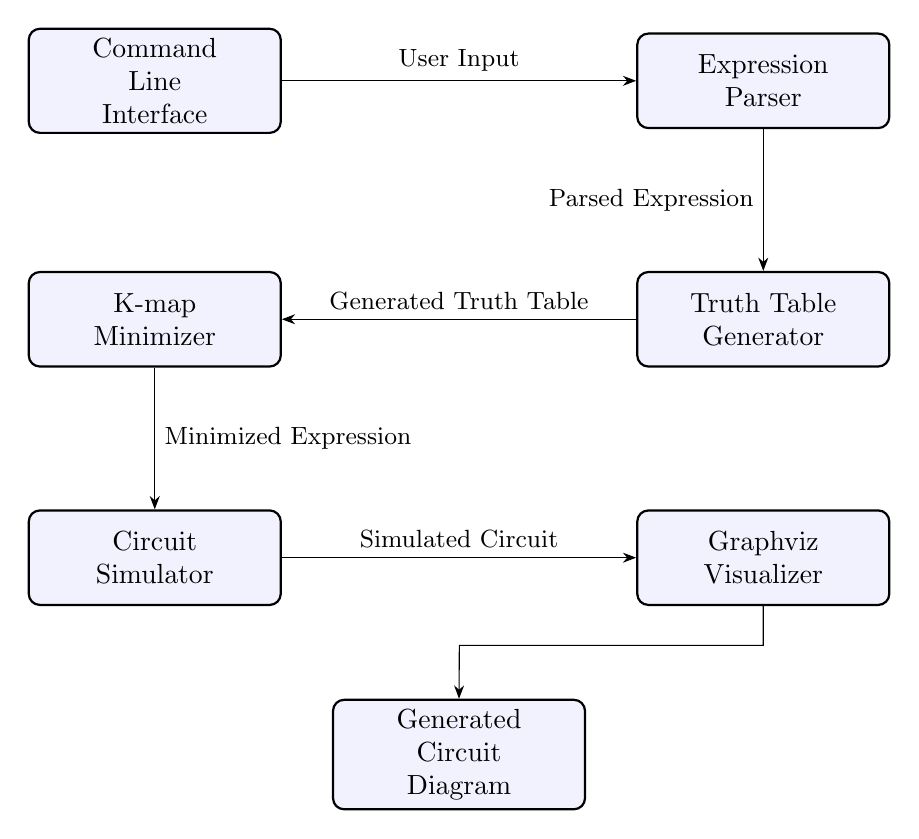
\begin{tikzpicture}[
  node distance=1.8cm and 4.5cm,
  box/.style={
    draw,
    rounded corners,
    minimum width=3.2cm,
    minimum height=1.2cm,
    align=center,
    fill=blue!5,
    thick
  },
  ->, >=Stealth
]

% First row
\node[box] (cli) {Command \\ Line \\ Interface};
\node[box, right=of cli] (parser) {Expression \\ Parser};

% Second row
\node[box, below=of parser] (ttg) {Truth Table \\ Generator};
\node[box, left=of ttg] (kmap) {K-map \\ Minimizer};

% Third row
\node[box, below=of kmap] (sim) {Circuit \\ Simulator};
\node[box, right=of sim] (viz) {Graphviz \\ Visualizer};

% Fourth row: center below sim and viz
\node[box] (cd) at ($(sim)!0.5!(viz) + (0,-2.5)$) {Generated \\ Circuit \\ Diagram};

% Arrows with labels
\draw (cli) -- node[midway, above] {\small User Input} (parser);
\draw (parser) -- node[midway, left] {\small Parsed Expression} (ttg);
\draw (ttg) -- node[midway, above] {\small Generated Truth Table} (kmap);
\draw (kmap) -- node[midway, right] {\small Minimized Expression} (sim);
\draw (sim) -- node[midway, above] {\small Simulated Circuit} (viz);

\draw[->] (viz.south) -- ++(0,-0.5) -- ++(-3.86,0) -- (cd.north);


\end{tikzpicture}
\caption{System Block Diagram of Digital Logic Suite}
\end{figure}

The overall architecture of the Digital Logic Suite can be represented by a block diagram showing how user inputs flow through different modules to produce outputs like truth tables, minimized expressions, simulated results, and visual diagrams.


\noindent The block diagram shows the following flow:
\begin{itemize}
    \item Users interact with the \textbf{Command-Line Interface (CLI)} to enter Boolean expressions or commands.
    \item The \textbf{Expression Parser} processes these expressions, checks syntax, and creates internal data structures.
    \item The \textbf{Truth Table Generator} uses the parsed expression to produce a complete truth table showing all input-output possibilities.
    \item The \textbf{Karnaugh Map Minimizer} takes the truth table and simplifies the logic using K-map techniques, generating minimized expressions.
    \item The \textbf{Circuit Simulator} uses the original or minimized expressions to simulate circuit behavior and outputs results.
    \item The \textbf{Graphviz Visualizer} generates visual diagrams of logic circuits and truth tables based on data from the parser, truth table, or minimizer.
\end{itemize}

This modular design ensures each component can operate independently while still contributing to the overall system, making the suite easy to develop, maintain, and extend.

\section{Methodology}

This project, “Digital Logic Suite,” is a C++ application that uses the SFML graphics library and follows object-oriented programming (OOP) ideas. We made different classes with private and public members to keep the code organized and safe. We used code reusability and data abstraction to make the project better. Each object has its own functions to handle events, and these work together to create the interactive simulation.

\vspace{0.5cm}
The Digital Logic Suite solves problems found in old digital logic simulators by giving users an easy-to-use tool made in C++ with SFML (Simple and Fast Multimedia Library). Unlike older tools that use only the command line, this simulator has a clear graphical interface. Users can see logic gates, circuit connections, and truth tables easily. By using OOP, we organized the code into classes, making it easier to reuse and maintain. Users can interact with the simulation, place components, and see how circuits work in real time. This makes it useful for learning and designing digital logic circuits.

\vspace{0.5cm}
Basic C++ graphics were not enough for our needs. To make a better and more interactive interface, we used SFML version 3.0.0. SFML gives us good graphics, works on different systems, and is easy to use for drawing, handling events, and getting input. We used VS Code as our IDE and the GCC compiler, which helped us code, compile, and debug on different platforms.

\vspace{0.5cm}
Before starting, we learned SFML by reading tutorials, official documents, and online guides. We also reviewed OOP concepts to design a system that is easy to manage. SFML is used for features like making the grid layout, simulating logic gates, showing the component palette, drawing the window, and creating buttons and the visual layout of the program.
\clearpage
\clearpage
\section{Project Scope}

The Digital Logic Suite is mainly created to help students, teachers, and anyone interested in learning about digital logic circuits. It is made for academic and educational purposes, so it focuses on providing clear and useful tools to understand how digital logic works.

This project provides a command-line interface (CLI) tool, which means users can type commands in a terminal or console to use the program. This makes the tool lightweight and easy to run on many different computers without needing a complex graphical interface.

The suite is designed to be modular. This means it is built in separate parts or modules that can work independently but also fit together smoothly. Because of this modular design, it will be easier to add new features or improve existing ones in the future without needing to rewrite the entire system.

The main focus of the Digital Logic Suite is on combinational logic, which is a type of digital logic where the output depends only on the current inputs. The tool will provide features to analyze these logic circuits, simplify or minimize the logic expressions to make them easier to understand and use, and simulate how the logic behaves with different inputs.

Overall, this project aims to be a simple, effective, and flexible tool that supports learning and experimentation in digital logic.


\clearpage
\section{Project Schedule}
\begin{table}[ht!]
    \centering
    \begin{tabular}{|>{\raggedright}p{2cm}|p{10cm}|}
        \hline
        \textbf{Week} & \textbf{Planned Activities}                                   \\
        \hline
        Week 1        & Requirements gathering, and system design.                    \\
        \hline
        Week 2        & Implementation of CLI and Boolean expression parser.          \\
        \hline
        Week 3        & Truth table generation and Karnaugh map minimization modules. \\
        \hline
        Week 4        & Circuit simulation and Graphviz visualization integration.    \\
        \hline
        Week 5        & Testing, documentation, and final report preparation.         \\
        \hline
    \end{tabular}
    \caption{Project Schedule for Digital Logic Suite}
\end{table}
\section{Libraries and Tools}
\begin{itemize}
    \item \textbf{C++ Standard Template Library (STL):} Utilized for object-oriented programming concepts and basic data structures.
    \item \textbf{Graphviz:} Visualization of logic circuits and truth tables.
    \item \textbf{Visual Studio:} Development environment.
    \item \textbf{Git:} Version control and collaboration.
\end{itemize}

\end{document}
